\documentclass{article}
\usepackage{geometry}
\geometry{left =3.0cm,right=3.0cm}
\usepackage{graphics}
\usepackage{indentfirst}
\usepackage{amsmath}
\usepackage{bm}
\usepackage{setspace}
\usepackage{graphicx}
\usepackage{float}
\usepackage{CJKutf8}
\author{Ruichen Wang}
\title{RL Introduction}
\begin{document}
\begin{CJK*}{UTF8}{gbsn}
\maketitle
\begin{abstract}
AI=RL+DL
\end{abstract}

\tableofcontents

\section{Basis}
\subsection{Introduction}
\textbf{Reinforcement learning} is learning what to do, how to map situations to actions, so
as to maximize a numerical reward signal. The learner must discover which actions yield the most reward by trying them. 

Of all the
forms of machine learning, reinforcement learning is the closest to the kind of learning
that humans and other animals do, and many of the core algorithms of reinforcement
learning were originally inspired by biological learning systems.

In the most interesting and challenging cases, actions may affect not only the immediate reward but also the next situation and, through that, all subsequent rewards.

Two most important distinguishing features:
\begin{itemize}
\item Trial and error search
\item Delayed reward
\end{itemize}

\begin{figure}[H]
\centering
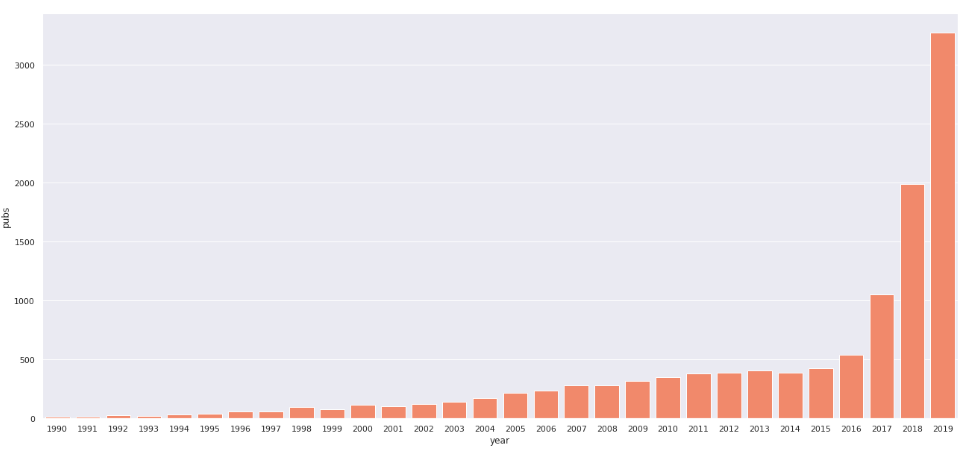
\includegraphics[width=6in,height=2.5in]{pub}
\caption{Publications by year}
\end{figure}

\subsection{Formalize Definition}
We formalize the problem of reinforcement learning using ideas from \textbf{dynamical systems theory}, specifically, as the optimal control of \textbf{incompletely-known Markov decision processes}.

Three key features:
\begin{itemize}
\item Sensation : sense the state of its environment to some extent
\item Action : take actions that affect the state
\item Goal : a goal or goals relating to the state of the environment
\end{itemize}

\begin{figure}[H]
\centering
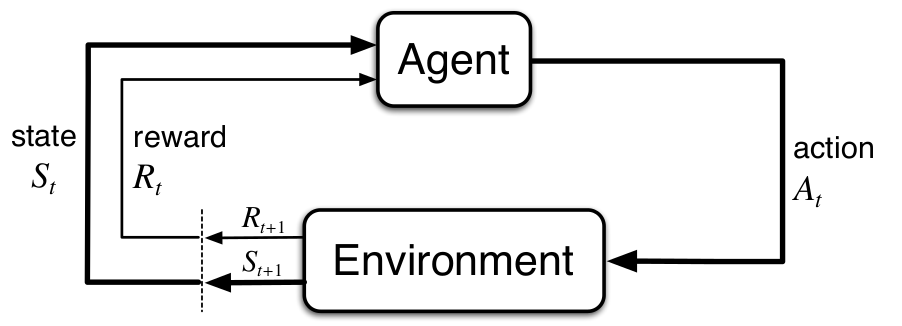
\includegraphics[width=6in,height=2in]{mdp}
\caption{MDP}
\end{figure}


\subsection{Difference Between Supervised or Unsupervised Learning}
In supervised learning, we have training set and labeled examples. In interactive problems it is often impractical to obtain examples of correct and representative behavior. An agent must be able to learn from its own experience.

In unsupervised learning, we aim to find structure hidden in collections of unlabeled data. Reinforcement learning is aiming to maximize a reward signal.

\begin{figure}[H]
\centering
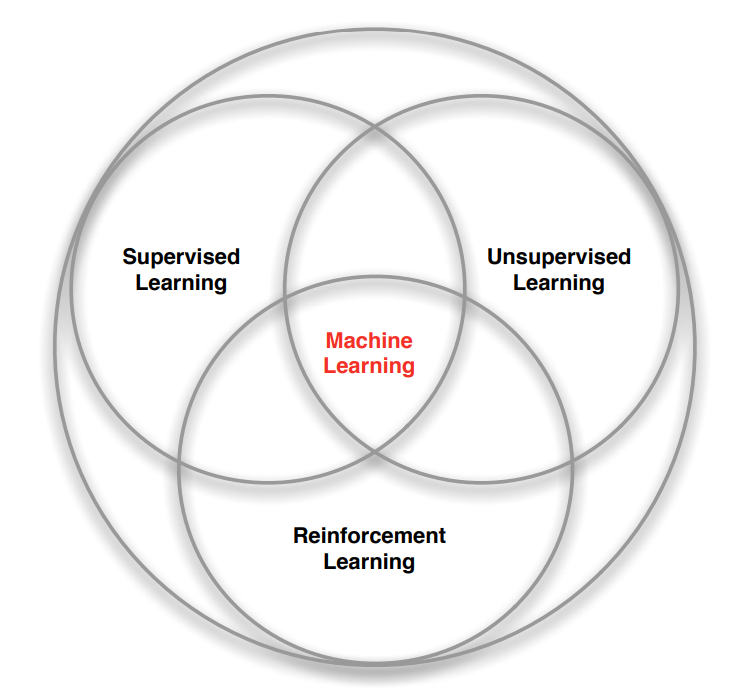
\includegraphics[width=4in,height=3.6in]{1}
\caption{Relationship}
\end{figure}

\subsection{Trade-off between Exploration and Exploitation}
The dilemma is that neither exploration nor exploitation can be pursued exclusively. We want the agent should be able to discover good policy without losing too much reward. Same important.


\section{Elements of Reinforcement Learning}
Beyond the \textbf{agent} and the \textbf{environment}, one can identify four main subelements of a
reinforcement learning system: a \textbf{policy}, a \textbf{reward signal} , a \textbf{value function}, and, optionally,
a \textbf{model of the environment}.


\subsection{Environment}
Environment can be classfied by whether its fully observable(MDP) or partially observable(POMDP).


\subsubsection{State,Observation and History}
A state $S$ is a complete description of the state of the world. There is no information about the world which is hidden from the state. An observation $O$ is a partial description of a state, which may omit information. A history $H$ is the sequence of observations, actions, rewards.
$$H_{t}=O_{1},R_{1},A_{1},...,A_{t-1},O_{t},R_{t}$$

State is a function of history. 
$$S_{t}=f(H_{t}) $$


*Markov state property: A state $S_{t}$ is Markov if and only if
$$P[S_{t+1}|S_{t}]= P[S_{t+1}|S_{1},...,S_{t}]$$

When the agent is able to observe the complete state of the environment, we say that the environment is fully observed. When the agent can only see a partial observation, we say that the environment is partially observed.
\newline
Fully observable:
$$O_{t}=S_{t}^{e}=S{t}^{a}$$
\newline
Partially observable:
$$S_{t}^{e}\neq S{t}^{a}$$
In this case, the agent must  construct its own state representation.
\subsection{Agent}

\subsubsection{Action}
Different environments allow different kinds of actions. The set of all valid actions in a given environment is often called the \textbf{action space}. 

Some environments have \textbf{discrete action spaces}, other environments have \textbf{continuous action spaces}. In continuous spaces, actions are real-valued vectors.


\subsection{Reward}
provided a \textbf{discounted rate} $\gamma$:
$G_{t}=R_{t}+\gamma R_{t+1}+\gamma^{2}R_{t+2}+...$

\subsection{Policy}
A map from state to action. Can be deterministic or stochastic.
$$a=\mu(s) \quad or \quad a \sim\pi(a|s)=P[A=a|S=s]$$

\subsection{Value function}
A prediction of future reward
\paragraph{State value function}
\begin{align*}
V_{\pi}(s_{t})=E_{\pi}[R_{t}|S_{t}=s_{t}] \\
= \sum_{a \in \forall} \pi(a|s)q_{\pi}(s,a) 
\end{align*}


\paragraph{Action-state value Function}

\begin{align*}
Q_{\pi}(s_{t},a_{t})=E_{\pi}[R_{t}|S_{t}=s_{t},A_{t}=a_{t}] \\
= \sum_{s^{'},r}p(s^{'},r|s,a)[r+\gamma * V_{\pi}(s^{'})]
\end{align*}


\paragraph{Bellman Expectation Equation}
\begin{align*}
V_{\pi}(s)=E_{\pi} [R_{t}+\gamma V_{\pi}(s_{t+1})|S_{t}=s_{t}] \\
= \sum_{a \ \in \ \forall} \pi(a|s) \sum_{s^{'},r}p(s^{'},r|s,a)[r+\gamma * V_{\pi}(s^{'})]
\end{align*}


\begin{align*}
Q_{\pi}(s_{t},a_{t})=E_{\pi}[R_{t}+\gamma Q_{\pi}(s_{t+1},a_{t+1})|S_{t}=s_{t},A_{t}=a_{t}]  \\
= \sum_{s^{'},r} p(s^{'},r|s,a)[r+\gamma * \sum_{a^{'} \in \forall} \pi(a^{'}|s^{'})q_{\pi}(s^{'},a^{'})]
\end{align*}


\paragraph{Optimal state value function}
$$V^{*}(s)=\max \limits_{\pi} V_{\pi}(s) $$

\paragraph{Optimal action-state value function}
$$Q^{*}(s,a)=\max \limits_{\pi} Q_{\pi}(s,a)$$

\paragraph{Bellman Optimal Equation}
$$V^{*}(s)=\max \limits_{a} Q^{*}(s,a) $$
$$Q^{*}(s,a)=\max \limits_{\pi} Q_{\pi}(s,a) = \sum_{s^{'},r}p(s^{'},r|s,a)[r+\gamma * V^{*}(s^{'})]$$

\subsection{Model}
A model predicts what the environemt will do next.
$$P_{next \; state}= P\left[s_{t+1}|s_{t},a_{t}\right]$$
$$R_{next \; reward}=R\left[r_{t+1}|s_{t},a_{t} \right]$$



\section{Model Free vs. Model Based}
One of the most important branching points in an RL algorithm is the question of whether the agent has access to (or learns) a model of the environment. By a model of the environment, we mean a function which predicts state transitions and rewards.

\begin{figure}[H]
\centering
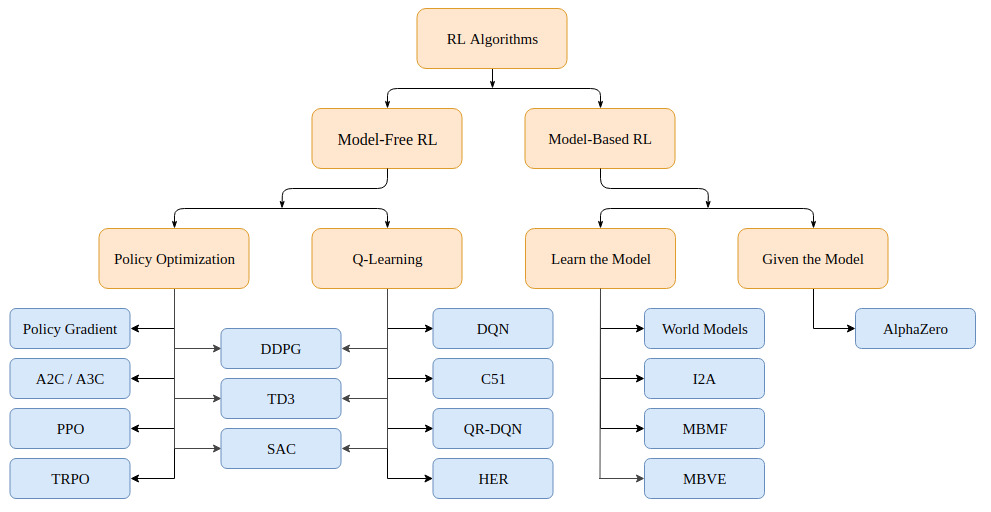
\includegraphics[width=5in,height=2.5in]{taxonomy2}
\caption{A Taxonomy of RL Algorithms}
\end{figure}

\subsection{Planning vs. Learning}
Two fundamental problems in sequential desicion making.


\begin{figure}[H]
\centering
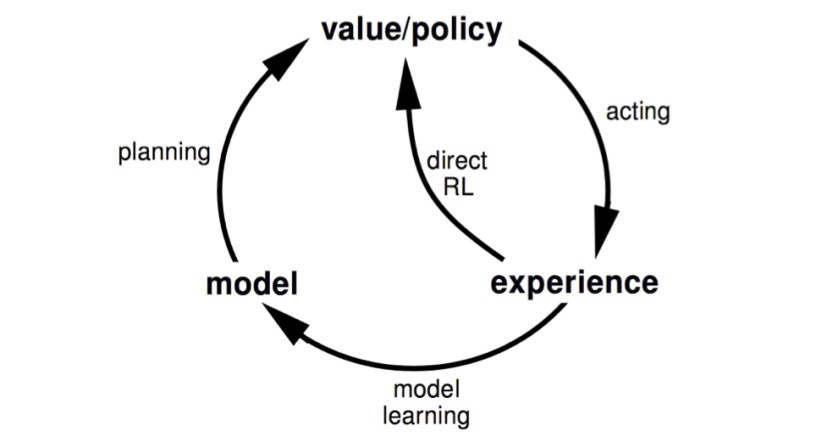
\includegraphics[width=3.5in,height=2in]{planning}
\caption{planning vs. learning}
\end{figure}


\begin{itemize}
\item Planning
\begin{itemize}
\item rule of environment is known
\item agent only perform with its model
\item agent improves policy
\end{itemize}
\item Learning
\begin{itemize}
\item environment unknow
\item agent directly interacts with environment
\item agent imporves policy
\end{itemize}
\end{itemize}


\subsection{Model Based}
Model based algorithm allows the agent to plan. Consider the problem as given MDP (S.A.R.T), 

using \textbf{policy iteration} or \textbf{value iteration} to solve the problem. Most rely on DP.
\begin{figure}[H]
\centering
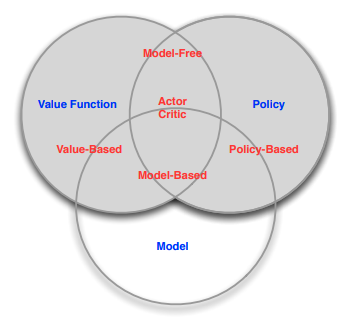
\includegraphics[width=4in,height=3.5in]{3}
\caption{Model free vs. model based}
\end{figure}


\subsection{Model Free}
The agent does not know how the world will change in response to its actions (the transition function  T ), nor what immediate reward it will receive for doing so (the reward function  R ).

The agent will simply have to try taking actions in the environment, observe what happens, and somehow, find a good policy from doing so.

How? MC, TD...

\subsubsection{Value-Based Reinforcement Learning}
Suppose we already know $Q^{*}(s_{t},a_{t})$, It is easy to choose which action to make. DQN is one way that using a neural network $Q(s;a;w)$ to approximate $Q^{*}(s_{t},a_{t})$. 

This optimization is almost always performed \textbf{off-policy}, which means that each update can use data collected at any point during training, regardless of how the agent was choosing to explore the environment when the data was obtained. 

\begin{align*}
Q(s_{t};a_{t};w) = r_{t}+\gamma \cdot Q(s_{t+1};a_{t+1};w) \\
= r_{t}+\gamma \cdot \max \limits_{a} Q(s_{t+1};a;w)
\end{align*}

Off policy : Q-learning. On policy: SARSA

\begin{figure}[H]
\centering
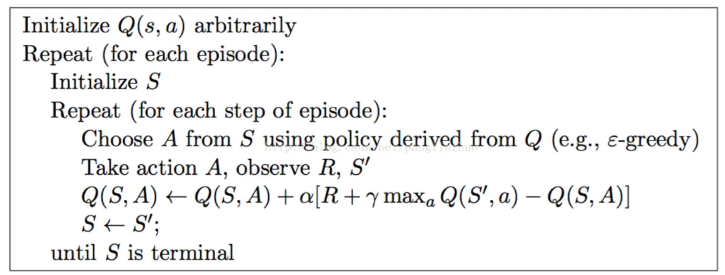
\includegraphics[width=6in,height=2in]{ql}
\caption{Q-learning}
\end{figure}


\begin{figure}[H]
\centering
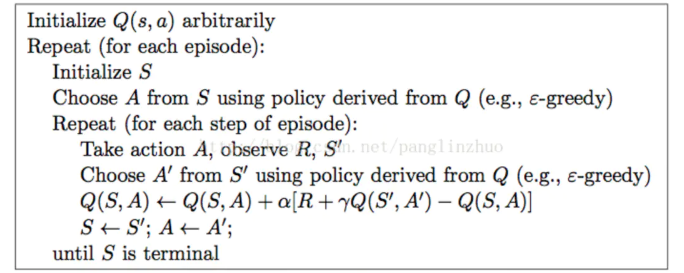
\includegraphics[width=6in,height=2in]{sarsa}
\caption{SARSA}
\end{figure}

\subsubsection{Policy-Based Reinforcement Learning}

Use a neural network $\pi(a|s;\theta)$ to approximate $\pi(a|s)$.

The goal of reinforcement learning is to find an optimal behavior strategy for the agent to obtain optimal rewards. The policy gradient methods target at modeling and optimizing the policy directly.

 This optimization is almost always performed \textbf{on-policy}, which means that each update only uses data collected while acting according to the most recent version of the policy.

\begin{align*}
V(s_{t};\theta) = \sum_{a \ \in \  \forall}\pi(a|s_{t};\theta)\cdot Q_{\pi}(s_{t},a_{t}) \\
= \int \pi(a|s_{t};\theta) \cdot Q_{\pi}(s_{t},a_{t}) da
\end{align*}
Policy gradient ascent to get max $J(\theta)$
$$J(\theta)=E_{S}[V(S;\theta)]=\sum_{s}V_{\pi}(s;\theta)$$

On Policy : REINFORCE, TRPO, PPO. 
Off Policy: DPG, Off-Policy Actor-Critic
\subsubsection{Trade-offs between Policy-based and Value-based}

Policy optimization methods
\begin{itemize}
\item  directly optimize for the thing you want
\item  stable and reliable. 
\end{itemize}


 
 Value-based methods 
 \begin{itemize}
 \item indirectly optimize for agent performance, by training $Q$ to satisfy a self-consistency equation. 
 \item tends to be less stable
 \item sample efficient, can reuse data more effectively than policy optimization
 \end{itemize}

 



\end{CJK*}
\end{document}
































